\chapter{Evaluation}
\label{chapter:evaluation}

For the evaluation of the approach the same six criteria from VIBES are taken: correctness, speed, scalability, flexibility, extensibility and powerful visuals. These criteria must be at least maintained or improved. Additionally, new use cases are showcased.

\section{Correctness}
The evaluation of the correctness of the simulator's frontend output is essential. By validating the output of the frontend we also validate the output of the backend.

Some parts of the evaluations are sample testing for consistency between the input parameters, expected and simulated or calculated output. Other parts are empirically tested.

For the calculation of the probability of a successful double spend and the maximal safe transaction value sample testing is used. For validating the success probability of simulated double spends empirical testing is applied.

\subsection{Block Size Limit}

\subsubsection{Average block size =< Non-SegWit maximal block size}

\subsubsection{Total number of processed transactions =< Non-SegWit maximal transactions per block * Blocks}

\subsection{Segregated Witness}

\subsubsection{Average block size =< SegWit maximal block weight =< SegWit theoretical block weight limit}

\subsubsection{Total number of processed transactions =< SegWit maximal transactions per block * Blocks}

\subsection{Simulated and Expected Transaction Incentives}
If the number of process transactions per block is smaller than the maximum number of transactions per block, then the transaction incentives have no impact. For the evaluation of transaction incentives we take a look at the Figures \ref{fig:TransactionIncentives1}, \ref{fig:TransactionIncentives2} and \ref{fig:TransactionSpam} which are all based on scenarios with full blocks.

\subsubsection{Transactions with higher fees should have a better confirmation status}
The first expectation is transaction with higher transaction fees should have preference over transaction with lower transaction fees, therefore in the transaction confirmation status chart the lower transaction fees should have a higher percentage of unconfirmed transactions. The simulated results confirm this expectation.

\subsubsection{Transactions with higher fees should have a shorter average transaction confirmation time}
The second expectation is transactions with higher transaction fees should have a shorter average transaction confirmation time. The simulated results confirm this expectation.

\subsection{Transaction Spam}
The Screenshot Transaction Spam \ref{fig:TransactionSpam} shows the simulated results which match the following expected results.

\subsubsection{No transaction confirmed with transaction fee below the target}
No transaction below the target transaction fee is expected. The charts about the transaction confirmation status and the average transaction confirmation time and the flood attack summary show that no confirmed transaction has a transaction fee below the target.

\subsubsection{All blocks are full}
One of the requirements of a transaction spam attack is that the blocks need to be full to block the transactions with fees below the target. All blocks in Figure \ref{fig:TransactionSpam} are full, except for the genesis block. There are 28 blocks, the maximum number of transactions per block is 100, so 2.700 transactions are expected and simulated.

\subsubsection{Flood attack transaction buffer is not shrinking}
To guarantee that no transaction below the target is confirmed, the flood attack transaction buffer should not decrease and stay constant. The number of pending flood attack transactions stays constant in the pending transaction chart.

\subsection{Expected and Simulated Transactions per Second}

For the evaluation of correctness of the transactions per second (tps) of our simulation, the formula for the calculation of \textit{tps} is compared to the implementation.

\begin{equation}
\text{tps} = \text{transactions per block} / \text{block time}
\end{equation}

Since the \textit{tps} for the whole simulation is an important key metric, the division is not done for one block, but instead for all blocks.

\begin{minipage}{\linewidth}
\begin{lstlisting}[style=myScalastyle]
    var tps: Double = longestChainNumberTransactions.toDouble / secondsBetween(VConf.simulationStart, VConf.simulateUntil).getSeconds.toDouble
\end{lstlisting}
\end{minipage}

As can be seen, the formulas are identical and therefore the result should be correct. Sample testing is done to check for implementation errors.

\subsubsection{Sample with a Simulation Duration of Six Hours}

For the first sample a short simulation of six hours is chosen. The chosen block time is 567 seconds and the chosen throughput is 105 transactions per block (\textit{tpb}).

Calculation of the expected total processed transactions \textit{pt}:
\begin{equation}
\textit{pt} = 6 \text{h} / 567 \text{sec} * 105 \text{tpb} = 6*60*60/567 * 105 = 4000
\end{equation}

Calculation of the expected \textit{tps}:
\begin{equation}
\text{tps} = 4000 \text{transactions} / 6 \text{h} = 0.185
\end{equation}

\begin{figure}[!htb]
\centering
\includegraphics[height=0.3\textwidth]{"figures/Testing/tps 1".PNG}
\caption{Screenshot Transactions per Second - 6h Simulation Duration\label{fig:tpsSimulation6h}}
\end{figure}

\begin{table}[ht]
    \caption{Simulated and expected results of transactions per second: Sample with 6h simulation duration\label{table:tps6hsimulation}}
\centering
\begin{adjustbox}{width=0.8\textwidth}
    \begin{tabular}{| l | r | r |}
    \hline
    \textbf{Metric} & \textbf{Simulation} & \textbf{Expectation}\\ \hline
    Block time & 692 & 567\\ \hline
    Total number of processed transactions & 3000 & 4000 \\ \hline
    Transactions per second & 0.14 & 0.185\\ \hline
    \end{tabular}
\end{adjustbox}
\end{table} 

As can be seen in Table \ref{table:tps6hsimulation}, for such a short simulation the tps is off by about 30\%. One reason for this significant difference is the difference in the block time between the simulated and expected values. This can be due to variance. To reduce block time variance a longer simulation time is chosen as a second sample.

The parameters for reproduction can be found in Chapter \ref{6hoursURL}.

\subsubsection{Sample with a Duration of 48 Hours}

For the second sample a longer simulation of 48 hours is chosen. The chosen block time is still 567 seconds and the chosen throughput is also still 105 transactions per block (\textit{tpb}).

Calculation of the expected total processed transactions:
\begin{equation}
\text{pt} = 48h / 567 \text{sec} * 105 \text{tpb} = 48*60*60/567 * 105 = 32000
\end{equation}

Of course the expected tps stays the same, since only the simulation duration parameter has been changed.

\begin{figure}[!htb]
\centering
\includegraphics[height=0.3\textwidth]{"figures/Testing/tps 2".PNG}
\caption{Screenshot Transactions per Second - 48h Simulation Duration\label{fig:tpsSimulation48h}}
\end{figure}

\begin{table}[ht]
    \caption{Simulated and expected results of transactions per second: Sample with 48h simulation duration\label{table:tps48hsimulation}}
\centering
\begin{adjustbox}{width=0.8\textwidth}
    \begin{tabular}{| l | r | r |}
    \hline
    \textbf{Metric} & \textbf{Simulation} & \textbf{Expectation}\\ \hline
    Block time & 539 & 567\\ \hline
    Total number of processed transactions & 
31700 & 32000 \\ \hline
    Transactions per second & 0.18 & 0.185\\ \hline
    \end{tabular}
\end{adjustbox}
\end{table} 

It can be observed in the second comparative table \ref{table:tps48hsimulation}, that a longer simulation duration leads the simulated block time to be closer to the expected block time. As a result the simulated \textit{tps} is close to the expected value.

The parameters for reproduction can be found in Chapter \ref{48hoursURL}.

\subsection{Expected and Calculated Probability of a Successful Double-Spending Attack}
\label{subsection:evalCalcDoubleSpending}
The probability of a successful double-spending attack is tested with five samples and the results are compared to the Figure \ref{fig:doubleSpend} from the research paper \textit{Analysis of Hashrate-Based Double Spending} \cite{doublespending}.

The variable q stands for the hashrate, the variable n is the number of confirmations. The edge cases q = 2\% and n = 1, q = 2\% and n = 10, q = 50\% and n = 1 and q = 50\% and n = 10 are tested as well as the common case of q = 30\% and n = 6.

\begin{table}[ht]
    \caption{Expected and Calculated Probabilities of a Successful Double-Spending Attack\label{table:doubleSpendingSimulatedAndCalculatedSuccessProbability}}
\centering
\begin{adjustbox}{width=0.8\textwidth}
    \begin{tabular}{| l | r | r | r | r |}
    \hline
    \textbf{Sample} & \textbf{n} & \textbf{q} & \textbf{Calculated Probability} & \textbf{Expected Probability} \\ \hline
    a & 2 & 1 & 4\% & 4\% \\ \hline
    b & 2 & 10 & 0\% & 0\% \\ \hline
    c & 50 & 1 & 100\% & 100\% \\ \hline
    d & 50 & 10 & 100\% & 100\% \\ \hline
    e & 30 & 6 & 15.645\% & 15.645\% \\ \hline
    \end{tabular}
\end{adjustbox}
\end{table}

All mentioned test cases in Figure \ref{fig:testCases} match the expected result.

\begin{figure}[p]
\centering

\subcaptionbox{Sample with input: q = 2\% and n = 1}{\includegraphics[width=0.365\textwidth]{"figures/Testing/q 2 n 1".PNG}}%
\hfill % <-- Separation
\subcaptionbox{Sample with input: q = 2\% and n = 10}{\includegraphics[width=0.365\textwidth]{"figures/Testing/q 2 n 10".PNG}}%
\hfill % <-- Separation

\vskip\baselineskip

\subcaptionbox{Sample with input: q = 50\% and n = 1}{\includegraphics[width=0.365\textwidth]{"figures/Testing/q 50 n 1".PNG}}%
\hfill % <-- Separation
\subcaptionbox{Sample with input: q = 50\% and n = 10}{\includegraphics[width=0.365\textwidth]{"figures/Testing/q 50 n 10".PNG}}%
\hfill % <-- Separation

\vskip\baselineskip

\subcaptionbox{Sample with input: q = 30\% and n = 6}{\includegraphics[width=0.365\textwidth]{"figures/Testing/q 30 n 6".PNG}}%
\hfill % <-- Separation

\caption{Screenshots Success Probability of Double-Spending\label{fig:testCases}}
\end{figure}

\subsection{Expected and Calculated Maximal Safe Transaction Value}
For the test of the maximal safe transaction value the samples from the evaluation of the successful double spend probability are reused and compared to Figure \ref{fig:maximalSafeTransactionValue}.

The additional input parameters were:

\begin{itemize}
\item Attack duration: 20 Blocks
\item Discount on stolen goods: 1
\item Attacked merchants: 5
\item Block reward: 12.5 BTC
\end{itemize}

Compared to the \textit{Analysis of Hashrate-Based Double Spending} paper the block reward was updated from 25 BTC to the current block reward of 12.5 BTC. This means the maximal safe transaction values need to be doubled to compare them with the correct values.

\begin{table}[ht]
    \caption{Expected and Calculated Maximal Safe Transaction Values (MSTV)\label{table:doubleSpendingSimulatedAndCalculatedMSTV}}
\centering
\begin{adjustbox}{width=0.65\textwidth}
    \begin{tabular}{| l | r | r | r | r |}
    \hline
    \textbf{Sample} & \textbf{n} & \textbf{q} & \textbf{Calculated MSTV} & \textbf{Expected MSTV} \\ \hline
    a & 2 & 1 & 1199 BTC & 1200 BTC \\ \hline
    b & 2 & 10 & $\infty$ BTC & $\infty$ BTC \\ \hline
    c & 50 & 1 & 0 BTC & 0 BTC \\ \hline
    d & 50 & 10 & 0 BTC & 0 BTC \\ \hline
    e & 30 & 6 & 269 BTC & 269.5 BTC \\ \hline
    \end{tabular}
\end{adjustbox}
\end{table}

Ignoring minor rounding differences in samples (a) and (e), all test cases in Figure \ref{fig:testCases} match the expected result. The sample with $\infty$ BTC is a special case, the frontend displays $\infty$ BTC in the case of receiving 2,147,483,647 BTC which is the maximal possible 32-bit signed integer value. 2,147,483,647 BTC is much more than the hard supply limit of 21 million BTC.

\subsection{Expected and Simulated Success Probability of Double Spending}
\label{subsection:evalDoubleSpending}
The success probability for the scenario with q = 30\% and n = 6 is reused from Chapter \ref{subsection:evalCalcDoubleSpending}.

For the empirical testing of double-spending a script was used, it can be found in Chapter \ref{evalDoubleSpending} for reproduction. It starts the simulation, waits for a certain time to let the simulation finish and repeats this for a total of 100 times.

\begin{table}[ht]
\caption{Double-spending outcomes and their simulated and expected probabilities\label{table:doubleSpendingSimulatedAndExpected}}
\centering
\begin{adjustbox}{width=1\textwidth}
    \begin{tabular}{| l | r | r | r |}
    \hline
    \textbf{Outcome} & \textbf{Occurrences} & \textbf{Simulated probability} & \textbf{Expected probability} \\ \hline
    Attack neither successful nor failed & 45 & - & - \\ \hline
    Attack successful & 8 & 15.09\% & 15.645\% \\ \hline
    Attack failed & 47 & 84.91\% & 84.355\% \\ \hline
    \textbf{TOTAL} & \textbf{100} & \textbf{100\%} & \textbf{100\%} \\ \hline
    \end{tabular}
\end{adjustbox}
\end{table}

After counting the occurrences of the outcomes in the logfile, they were summarized in Table \ref{table:doubleSpendingSimulatedAndExpected}. All simulations were finished in the specified time. The undecided attacks are ignored for the calculation of the probabilities. It is assumed that the unfinished simulations have a similar probability distribution like the finished ones. The simulated probability of the double-spending attack is with 15.09\% very close to the expected probability of 15.645\%, which was calculated in Chapter \ref{subsection:evalCalcDoubleSpending}. Hereby is shown that the simulation of double-spending has the correct success probability.

\section{Speed}
To make sure there are no significant performance losses introduced by the implementation of bitcoin, we compare the simulation results from BBSS with VIBES.

\section{Scalability}
The block size limit, the block weight limit and the target transaction fee in the case of a flood attack are in $O(1)$ and do not effect the performance, except for requiring increasing memory if the throughput is higher than the maximal transactions per block.

For examining the effect of the hashrate in case of a double-spending attack on the scalability, multiple simulations were executed. Figure \ref{figure:limitations} show there is no significant difference in simulation duration because of a varying hashrate.

\begin{figure}
\centering
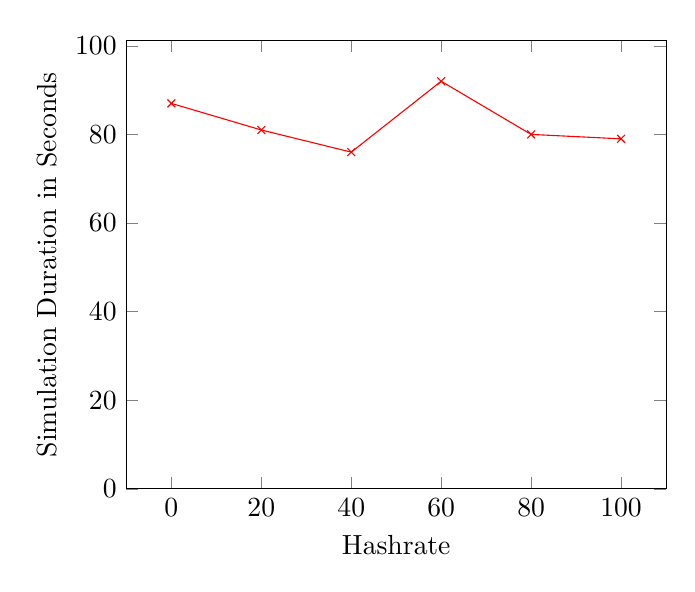
\begin{tikzpicture}
	\begin{axis}[
	    ymin=0,
		xlabel=Hashrate,
		ylabel=Simulation Duration in Seconds]
	\addplot[color=red,mark=x] coordinates {
		( 0,87)
		( 20,81)
		( 40,76)
		( 60,92)
		( 80,80)
		(100,79)
	};
	\end{axis}
\end{tikzpicture}
\caption{Effect of Hashrate on Simulation Duration\label{figure:limitations}}
\end{figure}

\section{Limitations of Speed and Scalability}
There are certain limitations on the simulator. One of the goals of the simulator is that the execution time of the simulation is shorter than the simulated duration. With increasing nodes and transactions, there is a point when the execution time equals the simulation time. In this chapter we want to examine this relationship and the resulting speedup ratio. The speedup ratio is the simulated duration divided by the execution duration.

All computations were done on a Home PC with Windows Ultimate 64-bit, Intel i7-4770 CPU @ 3.40 GHz and 16.0 GB 1600 MHz DD3.

The simulations were done with an equal number of nodes and transactions. This seems to be a good ratio for the simulator, which allows lots of parallel computation. 

The Table \ref{table:limitations} and the Figure \ref{figure:limitations2} shows the results of the simulations and the declining speedup ratio with increasing nodes and transactions. The values in the table should be considered as approximations, since only one simulation per number of nodes and transactions was done and the block time deviations can have an impact on the speedup ratio. One of the consequences deriving from this table is that it is not feasible to do a simulation with the configuration of the real-world bitcoin network with ten thousand nodes and one thousand tpb on a Home PC.

\begin{figure}
\centering
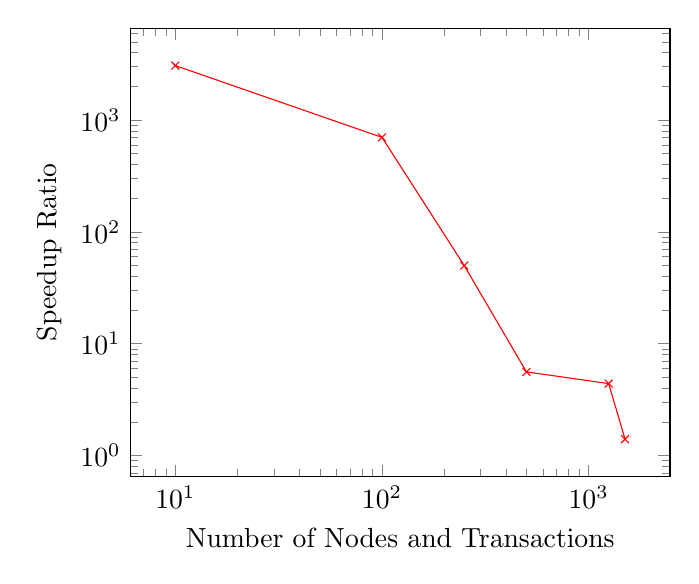
\begin{tikzpicture}
	\begin{loglogaxis}[
		xlabel=Number of Nodes and Transactions,
		ylabel=Speedup Ratio]
	\addplot[color=red,mark=x] coordinates {
		(  10,3070  )
		( 100, 700  )
		( 250,  50  )
		( 500,   5.6)
		(1250,   4.4)
		(1500,   1.4)
	};
	\end{loglogaxis}
\end{tikzpicture}
\caption{Effect of Hashrate on Simulation Duration\label{figure:limitations2}}
\end{figure}

\begin{table}[ht]
\caption{Effect of Number of Nodes and Transactions on the Speedup Ratio \label{table:limitations}}
\centering
\begin{adjustbox}{width=1\textwidth}
    \begin{tabular}{| r | r | r | r |}
    \hline
    \textbf{Number of Nodes and Transactions} & \textbf{Simulation Duration in Seconds} & \textbf{Execution Duration in Seconds} & \textbf{Speedup Ratio} \\ \hline
    10 & 21480 & 7 & 3070 \\ \hline
    100 & 21120 & 30 & 700 \\ \hline
    250 & 19140 & 373 & 50 \\ \hline
    500 & 6900 & 1228 & 5.6 \\ \hline
    1250 & 3045 & 697 & 4.4 \\ \hline
    1500 & 3060 & 2188 & 1.4 \\\hline
    \end{tabular}
\end{adjustbox}
\end{table}

Of course, other configuration parameters than nodes and transactions like block size limit or block weight limit have a limiting impact due to the increasing memory requirement.

\subsection{Realistic Bitcoin Network Simulation with AWS}

Amazon Web Service (AWS) is used to find out if it is actually possible to simulate a bitcoin network with ten thousand nodes and thousand tpb. The instance typ t2.2xlarge has a similar performance to the used Home PC and therefore doesn't have the required performance. The instance type p3.2xlarge was chosen, since it is advertised as "high performance computing" and as "ideal platform for technical simulations".

\begin{figure}[h]
\centering
\includegraphics[width=1\textwidth]{"figures/p32xlarge".PNG}
\caption{Screenshot AWS p3.2xlarge
\label{fig:aws}}
\end{figure}

Using various tools we asumme the following configuration parameters:
\begin{itemize}
\item strategy=BITCOIN\_LIKE\_BLOCKCHAIN
\item simulateUntil={1 hour}
\item blockTime=600
\item numberOfNeighbours=15
\item numberOfNodes=10000 \cite{configuration_node}
\item neighboursDiscoveryInterval=3000
\item latency=900
\item transactionSize=700 \cite{configuration_transaction_size}
\item maxBlockSize=0
\item throughput=1300 \cite{configuration_tpb}
\item transactionWeight=1400
\item maxBlockWeight=4000000
\item networkBandwidth=1
\item transactionPropagationDelay=150
\item hashRate=0
\item confirmations=0
\item transactionFee=0
\end{itemize}

With these configuration parameters the simulator uses only about 20\% CPU. This means realistic parameters do not allow lots of parallel computing. The number of neighbours seems to be too small, since the stale block rate is very high which leads slower than real-time simulation.

The numbers of neighbours needs to be between 19 and 22 to reach all nodes after four or five levels of block propagation. In VIBES the optimal number of neighbours for 100 nodes is 4 to 5 neighbours, which is a similar level of block propagation.

But with 21 neighbours the simulation is slower than real-time, the performance of p3.2xlarge is not sufficient. As shown in the Evaluation Chapter of VIBES, increasing the neighbours increases the execution time linearly. All these parameters like nodes, throughput and neighbours scale linearly, but put together they increase the execution effort too heavily.

\section{Flexibility}
asdf

\section{Extensibility}
asdf

\section{Powerful Visuals}

\begin{figure}[p]
\centering
\includegraphics[width=1\textwidth]{"figures/configuration".PNG}
\caption{Screenshot Configuration
\label{fig:configuration}}
\end{figure}

\begin{figure}[p]
\centering
\includegraphics[width=1\textwidth]{"figures/simulation-0-0".PNG}
\caption{Screenshot Simulation - Part 1
\label{fig:simulation1}}
\end{figure}

\begin{figure}[p]
\centering
\includegraphics[width=1\textwidth]{"figures/simulation-0-1".PNG}
\caption{Screenshot Simulation - Part 2
\label{fig:simulation2}}
\end{figure}

\section{Use Cases}
This thesis made new use cases possible, some of which are presented in the following chapter.

\subsection{Optimising Transactions per Second}
Scalability is one of the biggest issues of bitcoin-like blockchains. The simulator could be used to optimised the tps of bitcoin.

\cite{blocksizeincrease}

for example block size increase like in research paper..

\subsection{Securing a Blockchain Merchant}


\subsection{Choosing Transaction Fees}


\subsection{Flood Attack}
